\chapter{Diseño e implementación} % Main chapter title

\label{Chapter3} % Change X to a consecutive number; for referencing this chapter elsewhere, use \ref{ChapterX}

\definecolor{mygreen}{rgb}{0,0.6,0}
\definecolor{mygray}{rgb}{0.5,0.5,0.5}
\definecolor{mymauve}{rgb}{0.58,0,0.82}

%%%%%%%%%%%%%%%%%%%%%%%%%%%%%%%%%%%%%%%%%%%%%%%%%%%%%%%%%%%%%%%%%%%%%%%%%%%%%
% parámetros para configurar el formato del código en los entornos lstlisting
%%%%%%%%%%%%%%%%%%%%%%%%%%%%%%%%%%%%%%%%%%%%%%%%%%%%%%%%%%%%%%%%%%%%%%%%%%%%%
\lstset{ %
  backgroundcolor=\color{white},   % choose the background color; you must add \usepackage{color} or \usepackage{xcolor}
  basicstyle=\footnotesize,        % the size of the fonts that are used for the code
  breakatwhitespace=false,         % sets if automatic breaks should only happen at whitespace
  breaklines=true,                 % sets automatic line breaking
  captionpos=b,                    % sets the caption-position to bottom
  commentstyle=\color{mygreen},    % comment style
  deletekeywords={...},            % if you want to delete keywords from the given language
  %escapeinside={\%*}{*)},          % if you want to add LaTeX within your code
  %extendedchars=true,              % lets you use non-ASCII characters; for 8-bits encodings only, does not work with UTF-8
  %frame=single,	                % adds a frame around the code
  keepspaces=true,                 % keeps spaces in text, useful for keeping indentation of code (possibly needs columns=flexible)
  keywordstyle=\color{blue},       % keyword style
  language=[ANSI]C,                % the language of the code
  %otherkeywords={*,...},           % if you want to add more keywords to the set
  numbers=left,                    % where to put the line-numbers; possible values are (none, left, right)
  numbersep=5pt,                   % how far the line-numbers are from the code
  numberstyle=\tiny\color{mygray}, % the style that is used for the line-numbers
  rulecolor=\color{black},         % if not set, the frame-color may be changed on line-breaks within not-black text (e.g. comments (green here))
  showspaces=false,                % show spaces everywhere adding particular underscores; it overrides 'showstringspaces'
  showstringspaces=false,          % underline spaces within strings only
  showtabs=false,                  % show tabs within strings adding particular underscores
  stepnumber=1,                    % the step between two line-numbers. If it's 1, each line will be numbered
  stringstyle=\color{mymauve},     % string literal style
  tabsize=2,	                   % sets default tabsize to 2 spaces
  title=\lstname,                  % show the filename of files included with \lstinputlisting; also try caption instead of title
  morecomment=[s]{/*}{*/}
}


%----------------------------------------------------------------------------------------
%	SECTION 1
%----------------------------------------------------------------------------------------
\section{Análisis del software}

\subsection{Arquitectura del sistema}
La solución está integrada por seis componentes principales:

\begin{itemize}
\item Interfaz visual: diseñada en Unity3D, le permite al usuario interactuar con la aplicación.
\item Lógica .NET: es el backend de la interfaz visual, es la aplicación desarrollada en .NET utilizando CSharp como lenguaje de programación.
\item APIrest: a través de ella la aplicación embebida en el Hololens 2 se comunica con el servidor web.
\item Base de datos: es actualizada a través de la APIrest y almacena los parámetros del proceso \textit{batch}.
\item Comunicación OPC: envía los datos pertinentes al sistema de control a través del \textit{standard} industrial OPC.
\item Sistema de control: es representado por un controlador simulado.
\end{itemize}

En la figura \ref{fig:Diag_bloques} se puede observar el diagrama en bloques y la interacción entre los seis componentes principales.

\begin{figure}[htpb]
	\centering
	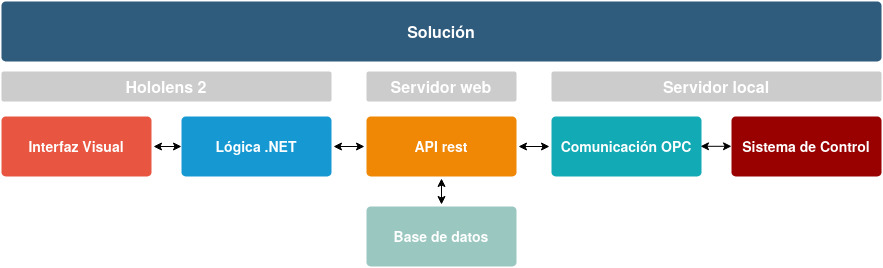
\includegraphics[scale=.5]{./Figures/Diag_bloques.jpg}
	\caption{Diagrama en bloques del sistema\protect\footnotemark.}
	\label{fig:Diag_bloques}
\end{figure}

\subsection{Interfaz visual y lógica .NET}

La aplicación embebida en el Hololens 2 se encarga de guiar al operador a través de todo el procedimiento \textit{batch}. En la figura \ref{fig:Flujo} se puede ver el diagrama de flujo.

\begin{figure}[htpb]
	\centering
	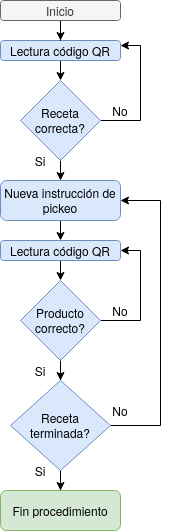
\includegraphics[scale=.7]{./Figures/Flujo.png}
	\caption{Diagrama de flujo\protect\footnotemark.}
	\label{fig:Flujo}
\end{figure}

En términos generales la aplicación se basa en la lectura de códigos QR para poder validar la operatoria del usuario. De esta manera, a lo largo del procedimiento se le solicitaran al operador distintas tareas las cuales tendrán asociadas un código QR especifico. Por ejemplo, para el agregado de un insumo al tanque de producción, se solicitara la lectura del código de la bolsa del insumo correcto para poder continuar. Mientras que en un proceso de transvase entre tanques, se le solicitara la lectura del código de la válvula que debe actuar para poder continuar. Como se muestra en la figura \ref{fig:Flujo}, mientras la lectura no sea correcta el operador no podrá avanzar de etapa.

A mas bajo nivel, cuando la aplicación inicia se instancia el objeto QRwatcher y el objeto Post. QRwatcher se ejecuta en \textit{background} para detectar la presencia de códigos QR en el ambiente, utilizando la cámara frontal del Hololens 2. Ademas crea una interfaz de servicio, para que el objeto Post se registre al mismo y reciba un \textit{handler} cuando ocurre una detección. El objeto Post se encarga de realizar las consultas a la API y crea el objeto Navegacion, este actualiza la información mostrada al operador durante todo el procedimiento. 

Luego de una detección, el \textit{handler} devuelve el dato codificado de la imagen QR y las coordenadas espaciales del código leído. Utilizando estas coordenadas se instancia un elemento holográfico, para indicar al operador si el código leído es correcto o incorrecto. Para esto se utilizo un tilde verde o una cruz roja sobre el código leído. De acuerdo con el tipo de lectura se dinamizan también botones alrededor del código. 

Utilizando los botones holográficos el operador puede cancelar la lectura o aceptarla. Si el código es incorrecto sólo podrá cancelar la lectura. Los botones tienen asociados eventos que disparan \textit{callbacks} al detectarse el pulsado. Si la lectura es correcta, el operador oprimirá aceptar y el \textit{callback} destruirá las instancias holográficas creadas, haciendo desaparecer los botones de la visual del operador. Al mismo tiempo, incrementa la variable de referencia \textit{steps}. Esta variable es publica del objeto Navegacion y se utiliza para determinar en que paso se encuentra la receta. El objeto Navegacion internamente implementa una maquina de estados para indicarle al operador las instrucciones correspondientes en cada etapa. 

En la etapa inicial, el objeto Post se encarga de ejecutar una consulta a la API y traer todos los parámetros de la receta leída. Estos parámetros se guardan en un objeto dataReceta el cual permanece inmutable durante toda la aplicación. Con estos datos, el objeto Navegacion es capaz de solicitar las instrucciones correctas en cada etapa e identificar cual seria el código requerido en cada una para poder avanzar. A continuación se muestra la maquina de estados del objeto Navegacion:

\begin{lstlisting}[label=cod:vControl,caption=Maquina de estados]  % Start your code-block

switch (steps)
{
	case 1:
   	textoinstruccion.GetComponent<TMPro.TextMeshProUGUI>().text = POST.dataReceta.msg1;
    break;
	
	case 2:
    _ = POST.PatchAsync("ValidationS1", "1");
    textoinstruccion.GetComponent<TMPro.TextMeshProUGUI>().text = POST.dataReceta.msg2;
    break;

	case 3:
    _ = POST.PatchAsync("ValidationS2", "1");
    textoinstruccion.GetComponent<TMPro.TextMeshProUGUI>().text = POST.dataReceta.msg3;
    break;

    case 4:
    _ = POST.PatchAsync("ValidationS3", "1");
    textoinstruccion.GetComponent<TMPro.TextMeshProUGUI>().text = POST.dataReceta.msgEnd;
    ButtonDatos.SetActive(false);
    canvas_proc.SetActive(false);
    ButtonMostrar.SetActive(false);
    MsgFin.SetActive(true);
    break;

    default:
    break;
}
\end{lstlisting}

La ventaja de esta solución es que el usuario puede modificar los códigos y las instrucciones requeridas sin interferir en la lógica de la aplicación dado que cada etapa se encuentra parametrizada con la información almacenada en la base de datos.

\subsection{API y base de datos}
La API (\textit{Application Programming Interface}) fue desarrollada en .NET y se implementaron las siguientes operaciones:

\begin{itemize}
\item GET: devuelve los datos de una receta.
\item POST: permite crear nuevas recetas.
\item PATCH: permite actualizar ciertos campos de la receta sin alterar el resto.
\item DELETE: elimina recetas de la colección.
\end{itemize}

Se creó una clase ``Receta'' la cual contiene los siguientes parámetros:

\begin{itemize}
\item id: número de identificación de la receta.
\item Receta: producto a fabricar.
\item Descripción: descripción del producto.
\item Status: running o stop, indica el estado de la receta.
\item Waitinput: sólo si esta en 1 la receta aguarda input del operador.
\item ValidationS1: 1 o 0 dependiendo si se cumplió la etapa del procedimiento.
\item ValidationS2: 1 o 0 dependiendo si se cumplió la etapa del procedimiento.
\item ValidationS3: 1 o 0 dependiendo si se cumplió la etapa del procedimiento.
\item ProductoP1: Nombre del producto de la etapa 1.
\item ProductoP2: Nombre del producto de la etapa 2.
\item ProductoP3: Nombre del producto de la etapa 3.
\item CodigoP1: Código del producto de la etapa 1.
\item CodigoP2: Código del producto de la etapa 2.
\item CodigoP3: Código del producto de la etapa 3.
\item CantidadP1: Cantidad del producto de la etapa 1.
\item CantidadP2: Cantidad del producto de la etapa 2.
\item CantidadP3: Cantidad del producto de la etapa 3.
\item Msg1: Mensaje para la etapa 1.
\item Msg2: Mensaje para la etapa 2.
\item Msg3: Mensaje para la etapa 3.
\item MsgEnd: Mensaje de fin de proceso.
\end{itemize}

Esta clase también se implementó en la lógica del Hololens 2. De esta manera, se utilizan los métodos GET y PATCH durante los pasos de la interfaz para adquirir o enviar datos a la API. Cuando desde la interfaz se lee un código QR internamente se envía una petición GET al servidor web para traer los datos de la receta y almacenarlos en una instancia de la clase Receta. Si la receta es correcta, se utiliza el mismo ID de receta para enviar las actualizaciones de estado cuando el operador avance una etapa. Esta actualización se hace con el método PATCH. Éste se implementó para modificar sólo los parámetros del input de usuario en la receta y no alterar el resto. 

La API se hosteo en Azure, la plataforma \textit{cloud} de Microsoft \citep{Azure}. Se utilizó el servicio Azure Web Apps \citep{WebApps}, que es una plataforma que permite publicar aplicaciones web que se ejecutan en múltiples \textit{frameworks} y escritas en diferentes lenguajes de programación. Esto permitió aumentar la velocidad de desarrollo de la aplicación dado que la sincronización y el \textit{deployment} son prácticamente instantáneos. Además, ofrece múltiples posibilidades de integración con otros servicios a futuro.

El motor de la base de datos utilizado es MongoDB \citep{mongo}. Es una base de datos NoSQL basada en documentos. Se optó por esta tecnología dado que los parámetros de las recetas podían ser encapsulados en un JSON. Se utilizó la plataforma SaaS de MongoDB, Atlas \citep{atlas}, para poder brindar flexibilidad y escalabilidad a la solución con una base de datos cloud. Para acceder a la misma se debe utilizar usuario y \textit{password}. La API es la única interfaz que posee esta información, por lo tanto puede realizar las operaciones CRUD \citep{CRUD} sobre la base de datos. A continuación se listan las operaciones:

\begin{itemize}
\item \textit{Create}: agrega nuevos documentos a la base de datos.
\item \textit{Read}: lee documentos de la base de datos.
\item \textit{Update}: actualiza los documentos existentes en la base de datos.
\item \textit{Delete}: borra documentos de la base de datos.
\end{itemize}

En la figura \ref{fig:dbpass} se puede ver el método de autenticación elegido en Atlas, para realizar las operaciones CRUD sobre la base de datos.

\begin{figure}[htpb]
	\centering
	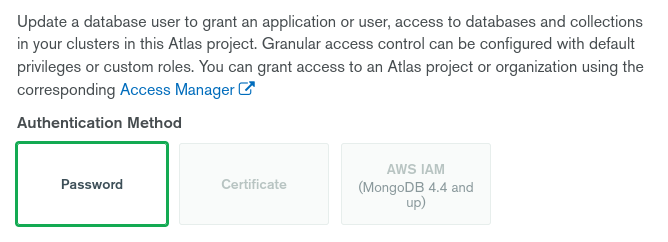
\includegraphics[scale=.5]{./Figures/dbpass.png}
	\caption{Método de autenticación elegido\protect\footnotemark.}
	\label{fig:dbpass}
\end{figure}

\subsection{Comunicación OPC}

Para la comunicación OPC se desarrollo un servicio y se instaló en el mismo nodo virtualizado en donde se ejecuta el sistema de control. Se encarga de actualizar la base de datos según los cambios en el sistema de control. Y viceversa, también es capaz de actualizar las variables de control de acuerdo a la base de datos. Se desarrolló en .NET y se ejecuta como un servicio más de Windows. El servicio incluye el \textit{framework} OPC mencionado en el Capítulo 2, lo que le permite leer y escribir variables OPC. A continuación podemos un extracto de código de la implementación de la interfaz OPC:

\begin{lstlisting}[label=cod:vControl,caption=Implementación de la interfaz OPC]  % Start your code-block

public interface IOpcClient : IDisposable
    {
        bool RefreshGruopAfterCreate { get; set; }
        bool LogSubcriptionsAndWrites { get; set; }
        bool IsServerRunning { get; }
        event ServerShutdownHandler OnServerShutdown;
        void Connect(bool createSubcription);
        void Connect();
        void Disconnect();
        object ReadObject(string idItem);
        string ReadString(string idItem);
        ushort ReadWord(string idItem);      
        void WriteString(string idItem, string value);
        void WriteWord(string idItem, ushort value);
    }
\end{lstlisting}

Podemos ver las funciones principales para leer y escribir, datos booleanos, strings y enteros del servidor OPC del sistema de control.

Una vez que el servicio se encuentra corriendo se encarga de realizar consultas GET a la APIrest de cada una de las recetas en ejecución. De ésta manera es capaz de detectar que los insumos ya fueron vertidos en el tanque y avanzar así a la siguiente etapa. Además, se encarga de setear la variable ``waitinput'', la misma es clave en el funcionamiento de la aplicación dado que indica que la receta se encuentra en ejecución y aguarda órdenes del operador. De ésta manera se valida que el operador sólo pueda iniciar la aplicación con la receta en ejecución por más que intente leer otros códigos de receta inválidos. 

\subsection{Sistema de control}

Este nodo se implementó en una máquina virtual usando VirtualBox, posee un sistema operativo Windows 10 con 4 gb de memoria RAM y 60 Gb de disco. La ventaja radica en la portabilidad del nodo, dado que podría integrarse a un servidor ESXI \citep{esxi} en cualquier entorno industrial. 

En el CBM podemos ver los bloques de las distintas recetas que se crearon en la aplicación de control, como se muestra en la figura \ref{fig:c7}.

\begin{figure}[htpb]
	\centering
	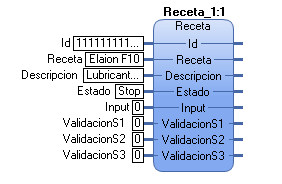
\includegraphics[scale=.6]{./Figures/c7.png}
	\caption{Bloque receta\protect\footnotemark.}
	\label{fig:c7}
\end{figure}

A medida que nuevas recetas sean necesarias, estos bloques funcionan como objetos de una clase que pueden instanciarse para cada tipo de receta. Simultáneamente estas recetas se cargan en la base de datos para establecer la comunicación entre el sistema de control y la interfaz del Hololens 2. Dentro de la receta se puede ver una lógica secuencial del procedimiento, que irá avanzando a medida que el operador complete los pasos en la interfaz holográfica. Podemos ver en la figura \ref{fig:c123} el avance de la secuencia en el tiempo.

\begin{figure}[htpb]
	\centering
	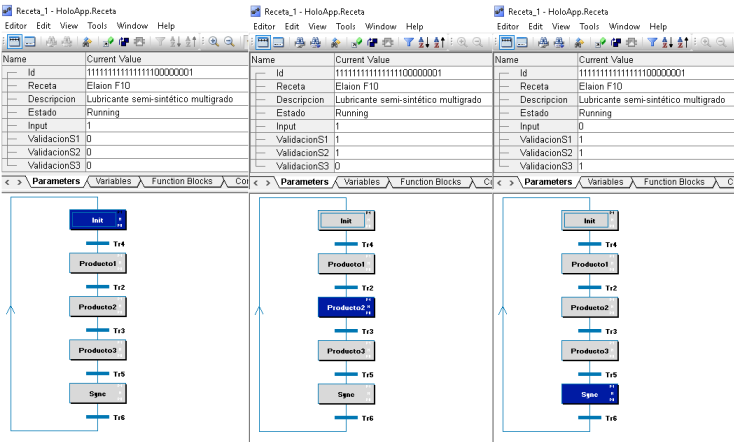
\includegraphics[scale=.5]{./Figures/c123.png}
	\caption{Secuencia\protect\footnotemark.}
	\label{fig:c123}
\end{figure}

La solución propuesta es fácilmente escalable desde la lógica de control y no esta atada a ningún proveedor en particular. Esto se debe a que en cualquier sistema de control somos capaces de crear este clase de objetos y comunicarlos vía el \textit{standard} OPC. Es por eso que el servicio OPC desarrollado, es capaz de operar con distintos sistemas de control sin alterar el funcionamiento de la aplicación desarrollada para el Hololens 2.

